\documentclass[12pt,a4paper]{article}

\usepackage[utf8]{inputenc}
\usepackage[T1]{fontenc}
\usepackage[brazil]{babel}
\usepackage{amsmath, amssymb, amsfonts}
\usepackage{geometry}
\usepackage{graphicx}
\usepackage{float}
\usepackage{booktabs}
\usepackage{siunitx}
\usepackage{listings}
\usepackage{xcolor}
\usepackage{hyperref}
\usepackage{caption}
\usepackage{enumitem}
\usepackage{physics}

\geometry{left=3cm,right=2cm,top=3cm,bottom=2cm}
\hypersetup{colorlinks=true, linkcolor=black, urlcolor=blue, citecolor=black}

\lstdefinestyle{pythonstyle}{
    language=Python,
    basicstyle=\ttfamily\small,
    keywordstyle=\color{blue},
    commentstyle=\color{teal!70!black},
    stringstyle=\color{red!70!black},
    numbers=left,
    numberstyle=\tiny,
    stepnumber=1,
    numbersep=8pt,
    showstringspaces=false,
    breaklines=true,
    frame=single,
    tabsize=4
}

\title{Solução Numérica do Problema de Condução Térmica 2D Transiente\\Formulação Implícita por Volumes Finitos}
\author{Gustavo Bittar Gonçalves}
\date{}

\begin{document}

\maketitle

\section{Enunciado resumido}
Considere uma chapa de aço AISI 304 com comprimento $L=\SI{0.02}{m}$ e espessura $e=\SI{0.01}{m}$, inicialmente a $\SI{30}{\celsius}$. Duas regiões da borda superior, definidas por $0.003 \le x \le 0.008$ e $0.012 \le x \le 0.017$, recebem subitamente um fluxo de calor uniforme de $q''=5\times 10^4\,\si{W/m^2}$. Nas demais fronteiras ocorre troca convectiva com o meio, adotando-se $T_{\infty}=\SI{30}{\celsius}$ e $h=\SI{20}{W/(m^2.K)}$. As propriedades térmicas são $k=\SI{14.9}{W/(m.K)}$ e $\alpha = 3.95\times 10^{-6}\,\si{m^2/s}$, e o tempo final da simulação é $t_{final}=\SI{60}{s}$.

Deseja-se determinar a distribuição de temperatura ao longo do tempo e construir os gráficos de $T\times t$ nas posições aproximadas $T(x=0.01,y=0,t)$, $T(x=0.01,y=0.005,t)$ e $T(x=0.01,y=0.01,t)$.

\section{Modelagem matemática}
Para condução bidimensional transiente com propriedades constantes e sem geração volumétrica interna, a equação governante é
\begin{equation}
\rho c_p \frac{\partial T}{\partial t} = k\left(\frac{\partial^2 T}{\partial x^2} + \frac{\partial^2 T}{\partial y^2}\right).
\end{equation}

Usando a relação
\begin{equation}
\alpha = \frac{k}{\rho c_p},
\end{equation}
obtém-se
\begin{equation}
\rho c_p = \frac{k}{\alpha}.
\end{equation}

As condições de contorno são:
\begin{align}
-k\pdv{T}{y} &= q'', &&\text{nas duas faixas aquecidas da borda superior},\\
-k\pdv{T}{n} &= h(T_s-T_{\infty}), &&\text{nas demais fronteiras com convecção},\\
T(x,y,0) &= T_0 = \SI{30}{\celsius}. &&
\end{align}

\section{Discretização por volumes finitos}
Integra-se a equação governante em um volume de controle retangular e utiliza-se uma formulação implícita no tempo. Para um volume genérico $P$, obtém-se
\begin{equation}
a_P T_P^{n+1} = a_E T_E^{n+1} + a_W T_W^{n+1} + a_N T_N^{n+1} + a_S T_S^{n+1} + b,
\end{equation}
em que
\begin{equation}
a_P = a_E + a_W + a_N + a_S + a_P^0 - S_P,
\end{equation}
com
\begin{equation}
a_P^0 = \frac{\rho c_p \Delta V}{\Delta t}.
\end{equation}

Para faces internas da malha, os coeficientes difusivos são
\begin{equation}
a_E = \frac{kA_e}{\delta x},\quad
 a_W = \frac{kA_w}{\delta x},\quad
 a_N = \frac{kA_n}{\delta y},\quad
 a_S = \frac{kA_s}{\delta y}.
\end{equation}

A contribuição das fronteiras convectivas é incorporada por linearização do tipo
\begin{equation}
S_P = -U,\qquad S_u = UT_{\infty},
\end{equation}
com
\begin{equation}
U = \frac{1}{R_{cond}+R_{conv}},
\end{equation}
\begin{equation}
R_{cond}=\frac{\Delta/2}{kA},\qquad R_{conv}=\frac{1}{hA}.
\end{equation}

Já o fluxo de calor imposto na borda superior entra como termo fonte
\begin{equation}
S_u = q''A_n.
\end{equation}

\section{Estratégia numérica}
Foi adotada uma malha uniforme com $N_x=41$ e $N_y=21$, de modo que os pontos de interesse ficassem representados com boa resolução. Em cada passo temporal, monta-se o sistema linear global e resolve-se
\begin{equation}
[A]\{T\}^{n+1}=\{b\}.
\end{equation}

O programa foi escrito para utilizar, quando disponível, um resolvedor iterativo de Jacobi em GPU via CUDA. Na ausência de GPU compatível, o algoritmo faz \emph{fallback} automático para processamento em série na CPU, preferencialmente usando o resolvedor esparso direto \texttt{spsolve}; se necessário, ainda existe um segundo \emph{fallback} para Jacobi em CPU.

\section{Código Python comentado}
O código abaixo monta o sistema por volumes finitos, resolve o problema no tempo, plota os gráficos relevantes e salva as figuras em formato PNG. O arquivo sugerido é \texttt{heat2d\_solver\_cuda\_fallback.py}.

\lstset{style=pythonstyle}
\lstinputlisting{heat2d_solver_cuda_fallback.py}

\section{Figuras a serem adicionadas ao documento}
Após executar o programa, as figuras serão salvas na pasta \texttt{figuras}. A seguir são mostrados exemplos de inclusão no relatório. Basta manter os nomes dos arquivos ou ajustá-los conforme necessário.

\subsection{Histórico temporal de temperatura}
A Figura~\ref{fig:historico} apresenta a evolução temporal da temperatura nos três pontos pedidos no enunciado.

\begin{figure}[H]
    \centering
    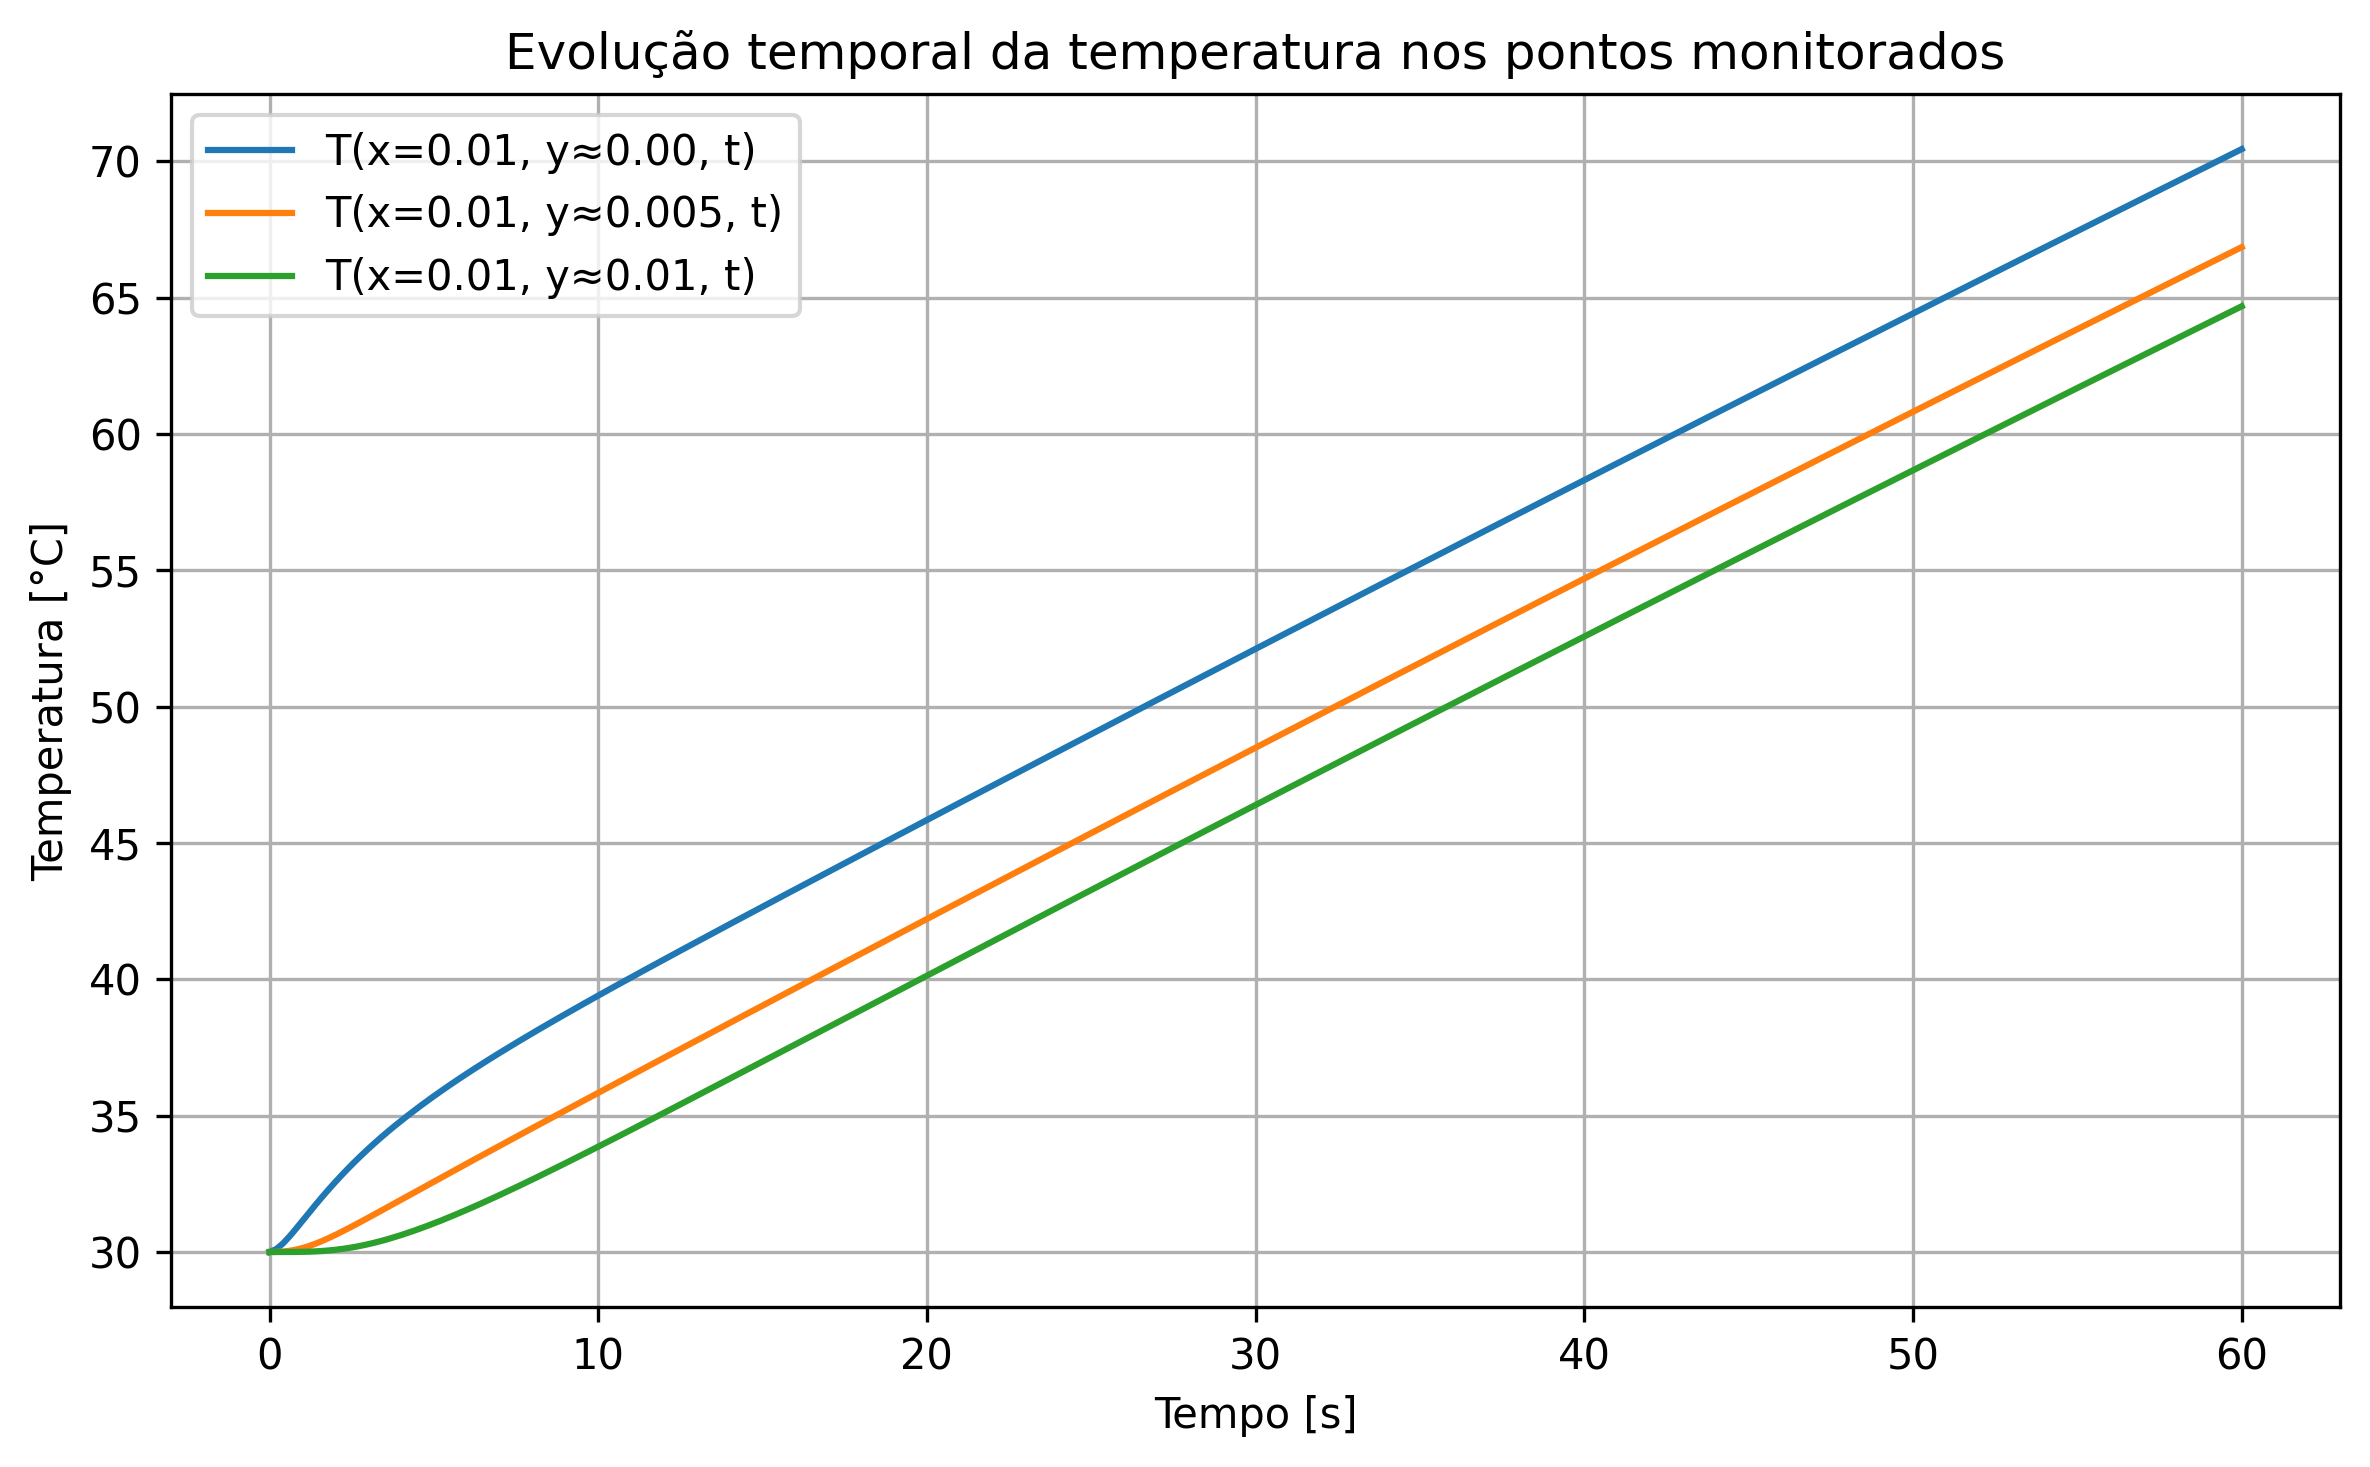
\includegraphics[width=0.82\textwidth]{figuras/historico_temperatura.png}
    \caption{Evolução temporal da temperatura nos pontos monitorados.}
    \label{fig:historico}
\end{figure}

\subsection{Campo de temperatura final}
A Figura~\ref{fig:campo-final} mostra o campo de temperatura no instante final da simulação, enquanto a Figura~\ref{fig:superficie-final} apresenta a superfície térmica correspondente.

\begin{figure}[H]
    \centering
    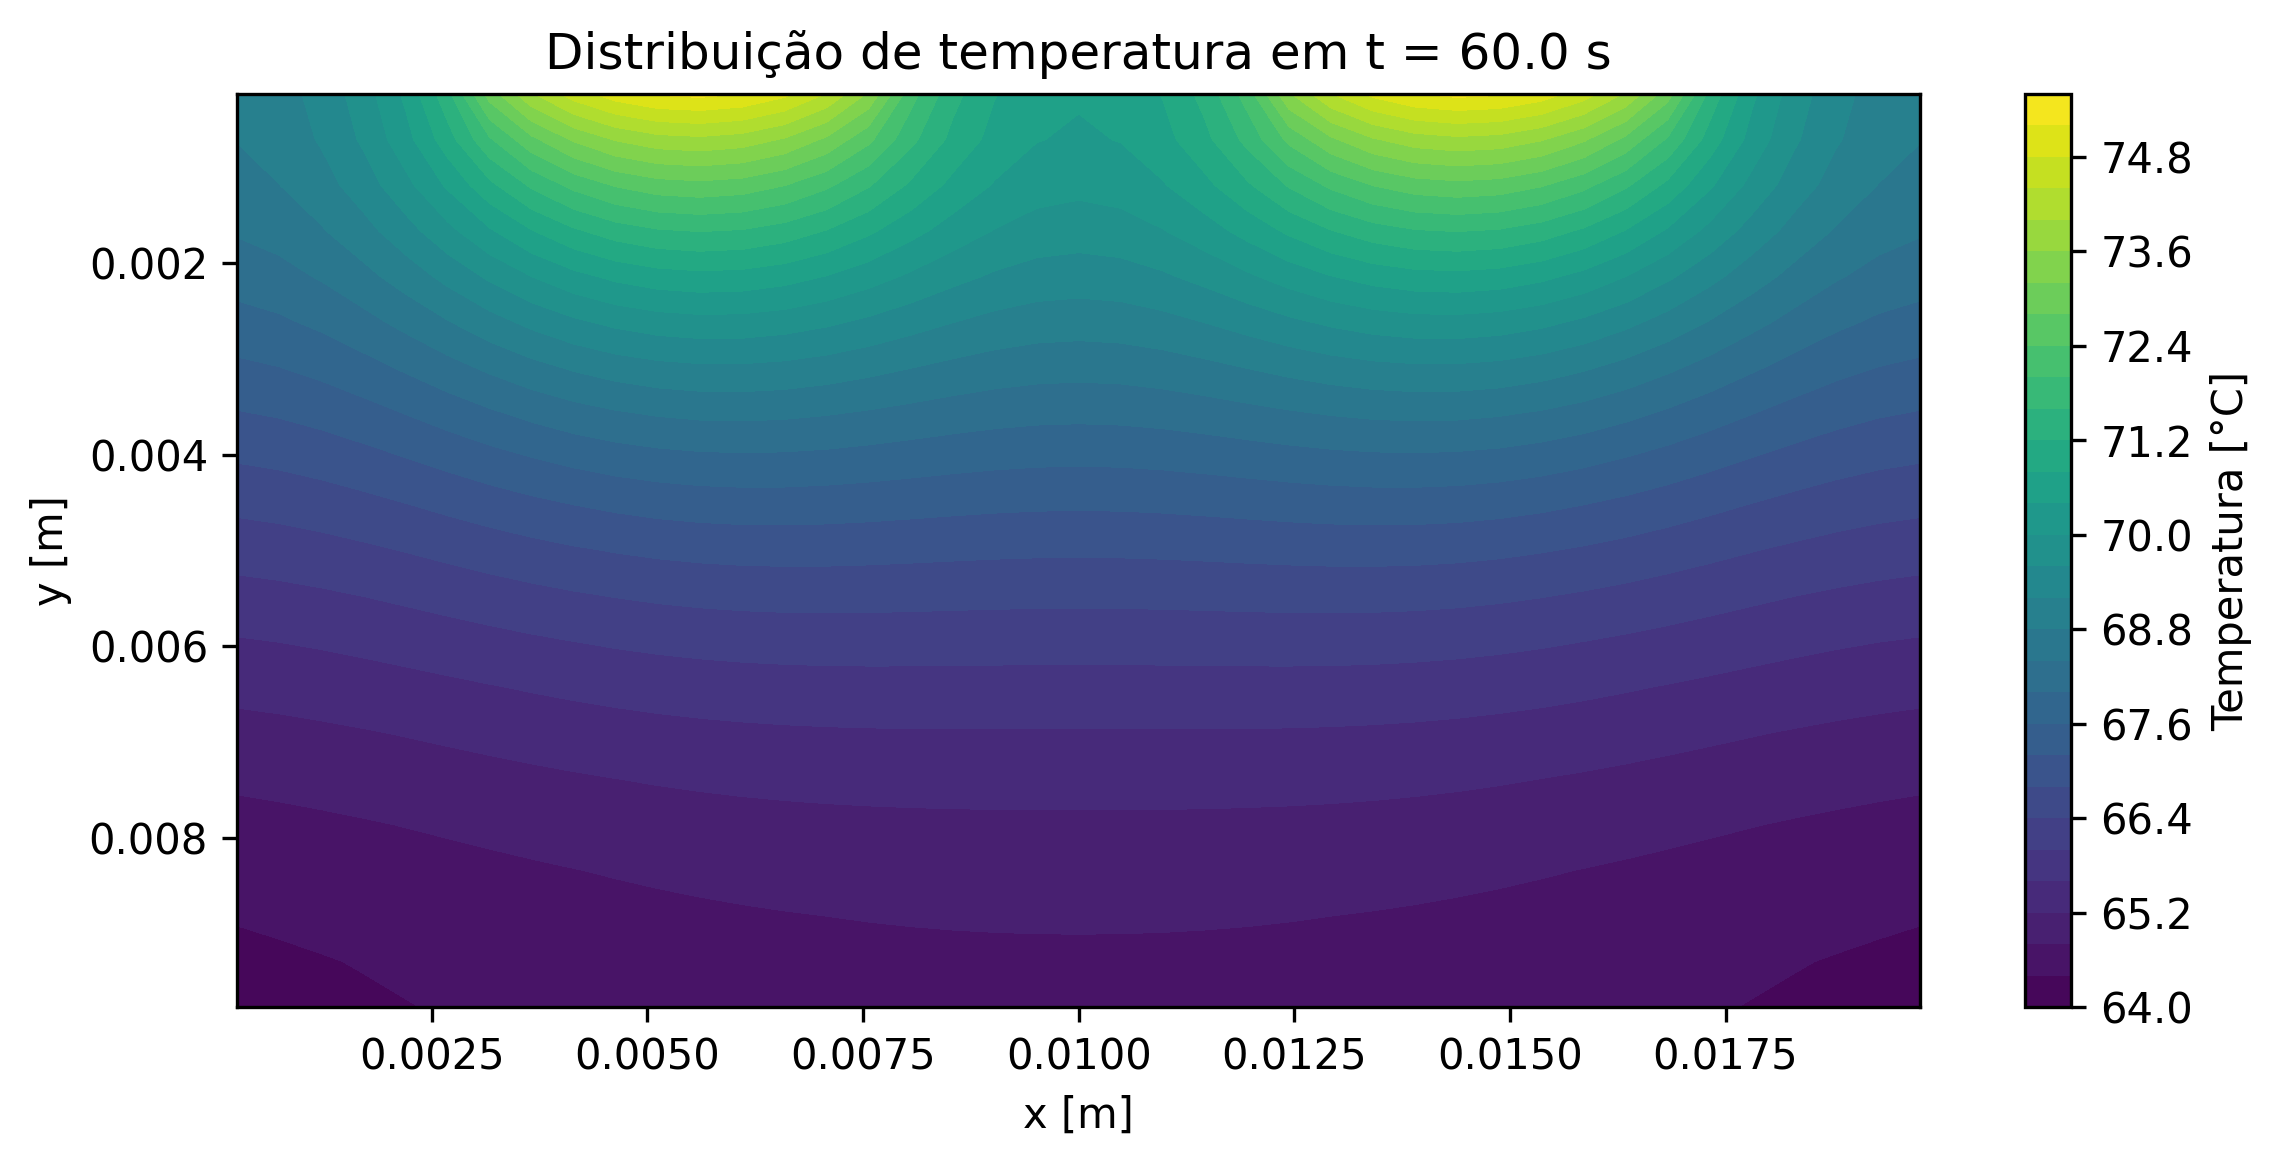
\includegraphics[width=0.82\textwidth]{figuras/campo_temperatura_final.png}
    \caption{Campo de temperatura em $t=\SI{60}{s}$.}
    \label{fig:campo-final}
\end{figure}

\begin{figure}[H]
    \centering
    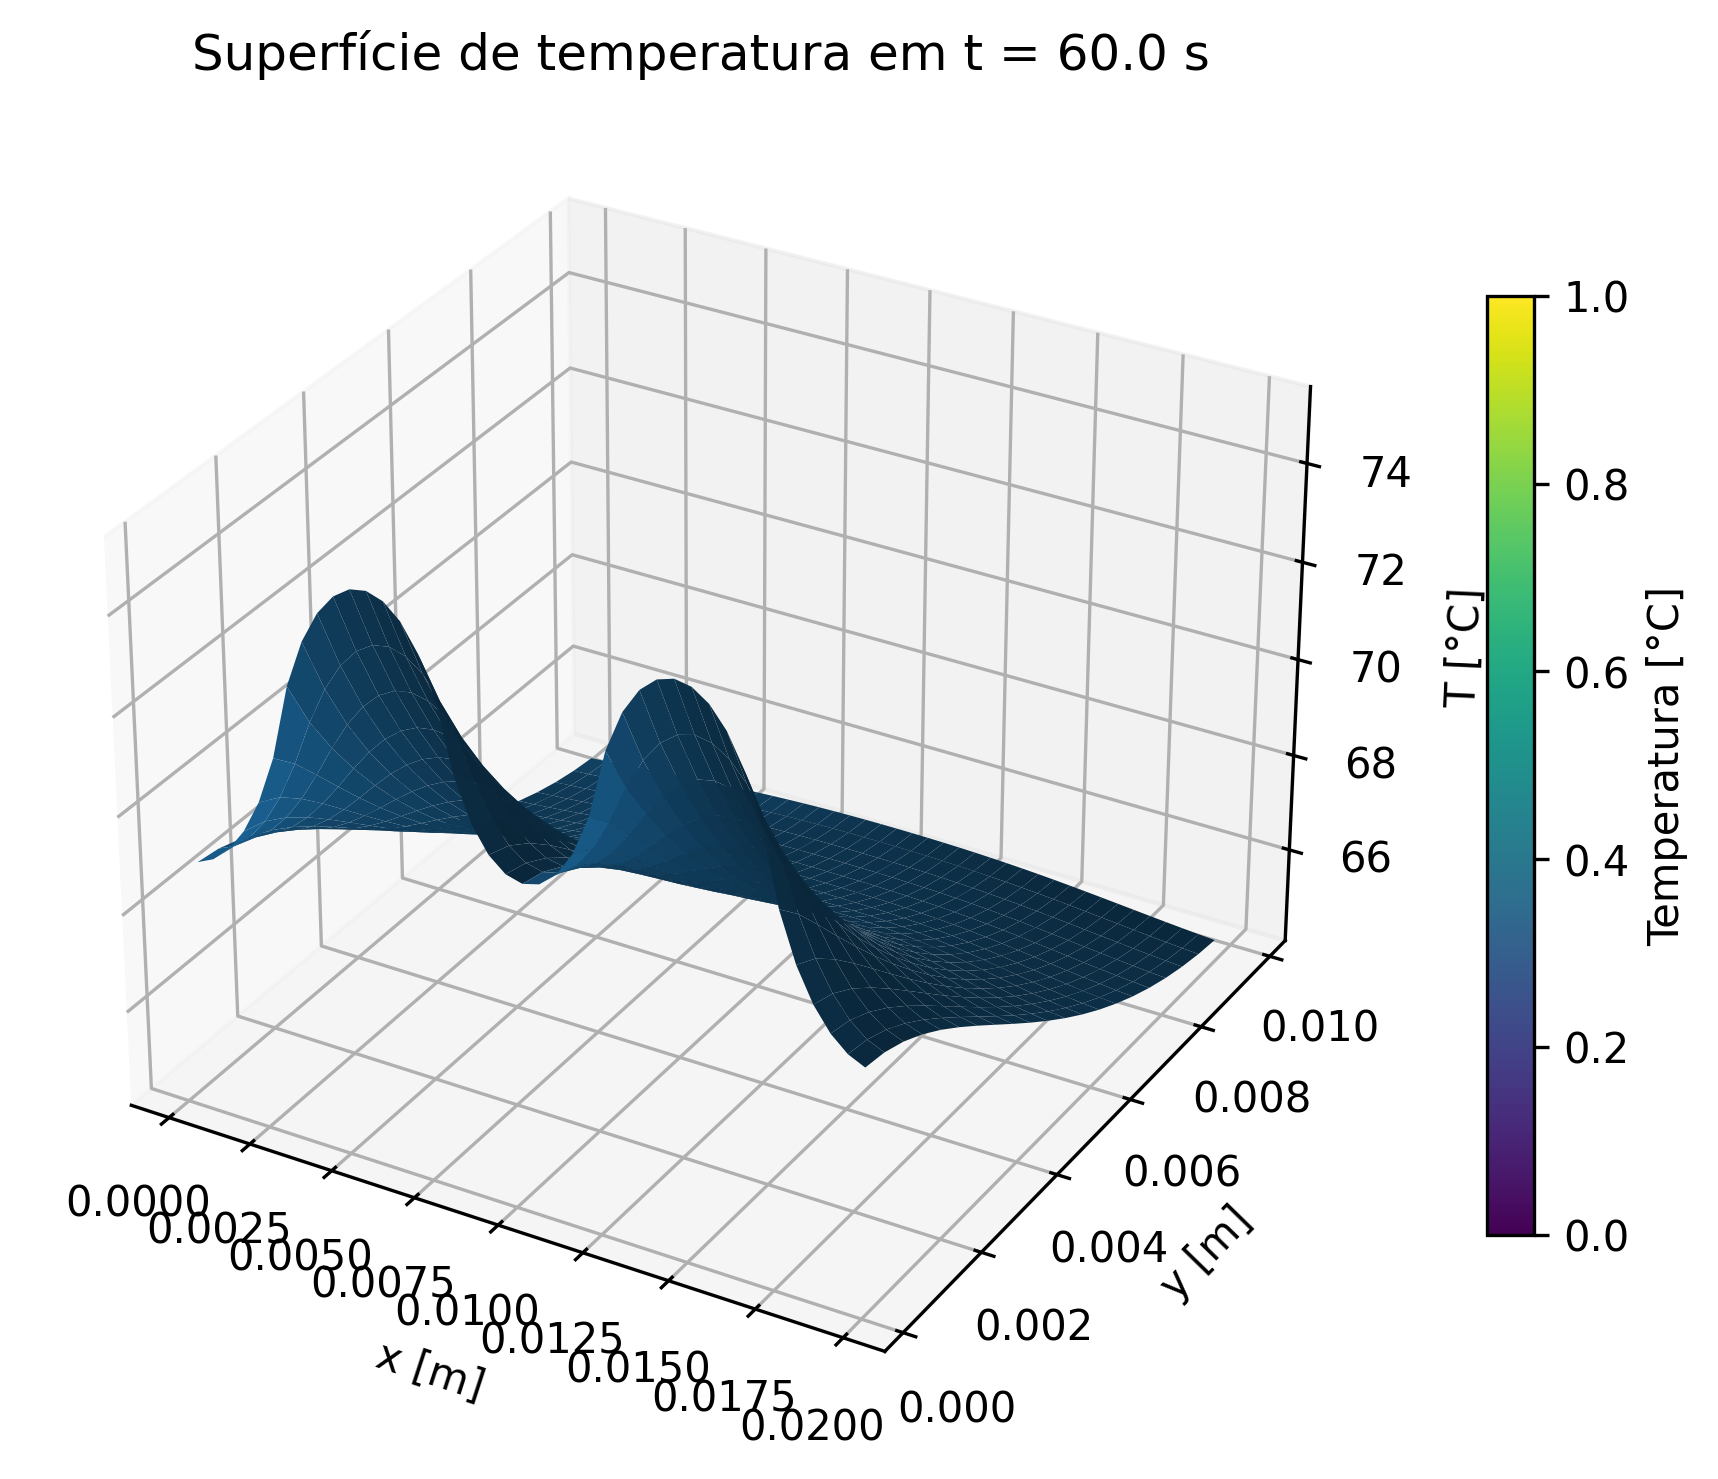
\includegraphics[width=0.82\textwidth]{figuras/superficie_temperatura_final.png}
    \caption{Superfície de temperatura em $t=\SI{60}{s}$.}
    \label{fig:superficie-final}
\end{figure}

\subsection{Campos intermediários}
As Figuras~\ref{fig:t0}, \ref{fig:t1}, \ref{fig:t5}, \ref{fig:t10}, \ref{fig:t30} e \ref{fig:t60} permitem visualizar a evolução do campo térmico ao longo do tempo.

\begin{figure}[H]
    \centering
    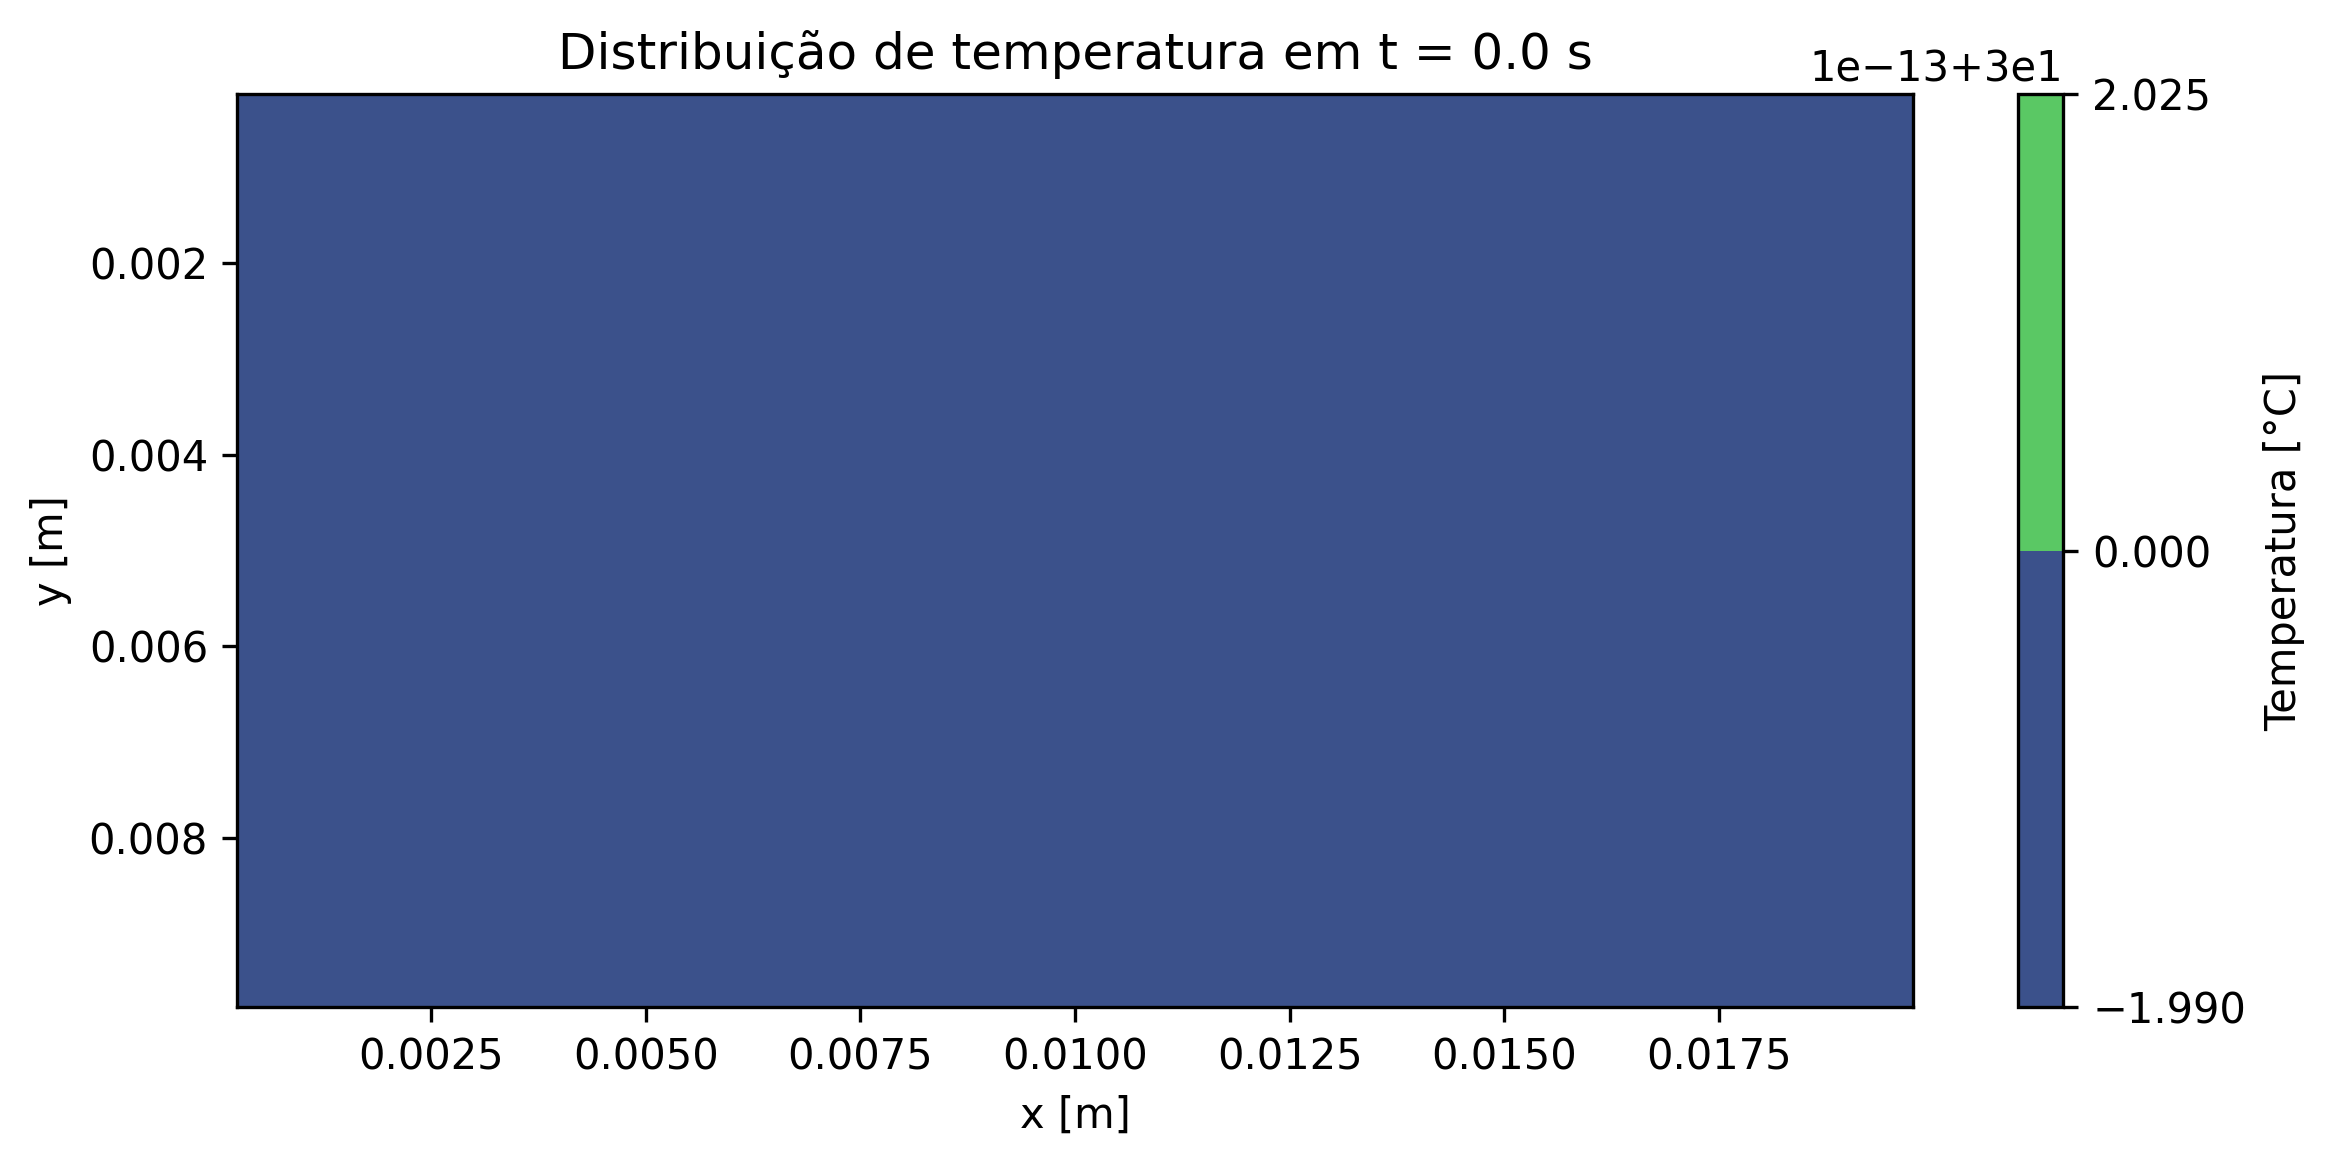
\includegraphics[width=0.78\textwidth]{figuras/campo_temperatura_t_0_0.png}
    \caption{Campo de temperatura em $t=\SI{0}{s}$.}
    \label{fig:t0}
\end{figure}

\begin{figure}[H]
    \centering
    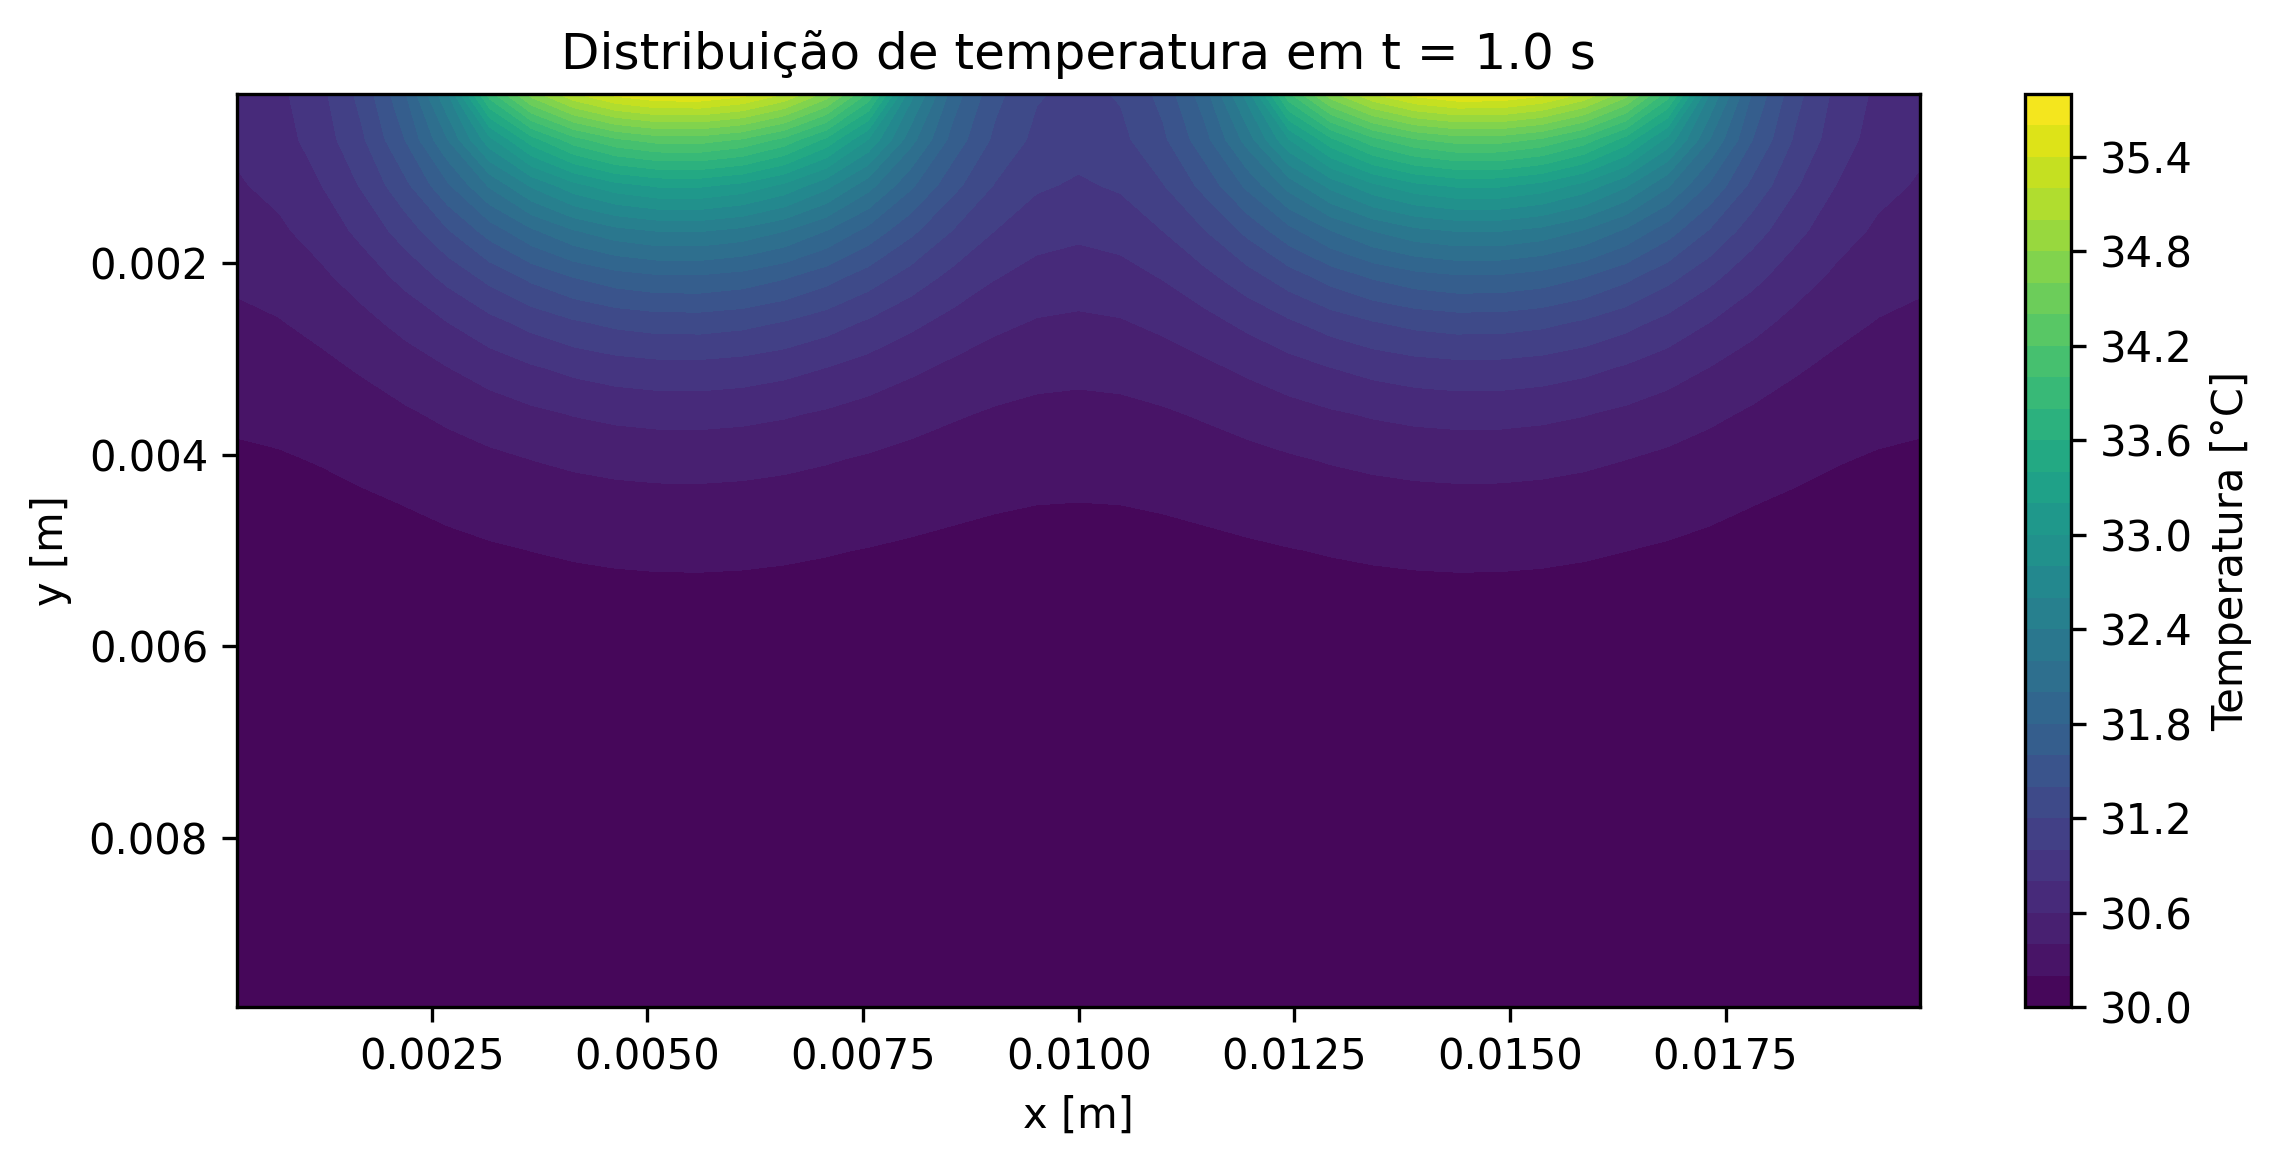
\includegraphics[width=0.78\textwidth]{figuras/campo_temperatura_t_1.png}
    \caption{Campo de temperatura em $t=\SI{1}{s}$.}
    \label{fig:t1}
\end{figure}

\begin{figure}[H]
    \centering
    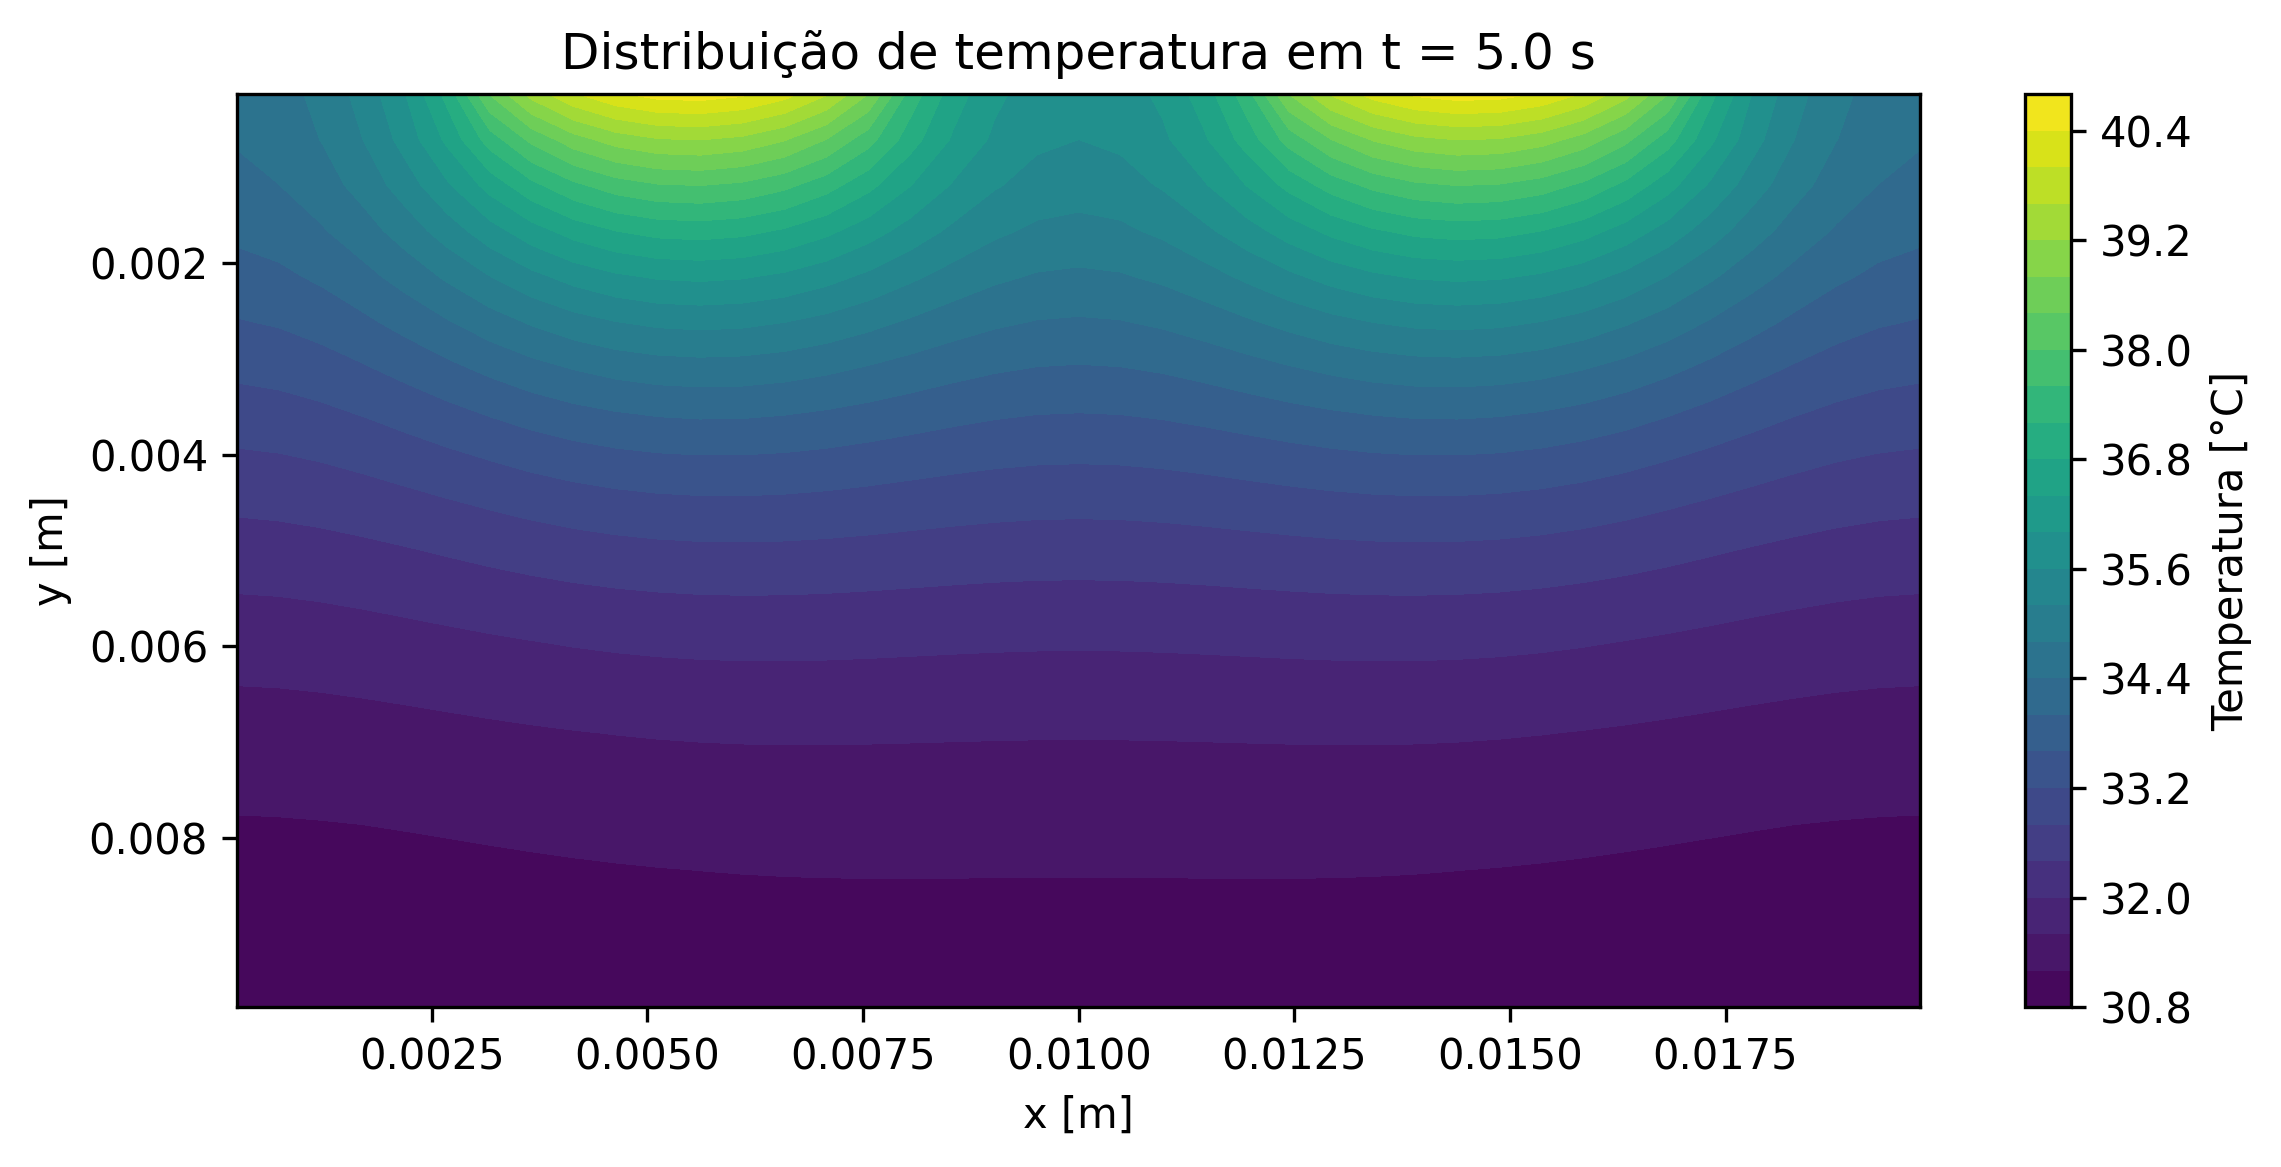
\includegraphics[width=0.78\textwidth]{figuras/campo_temperatura_t_5.png}
    \caption{Campo de temperatura em $t=\SI{5}{s}$.}
    \label{fig:t5}
\end{figure}

\begin{figure}[H]
    \centering
    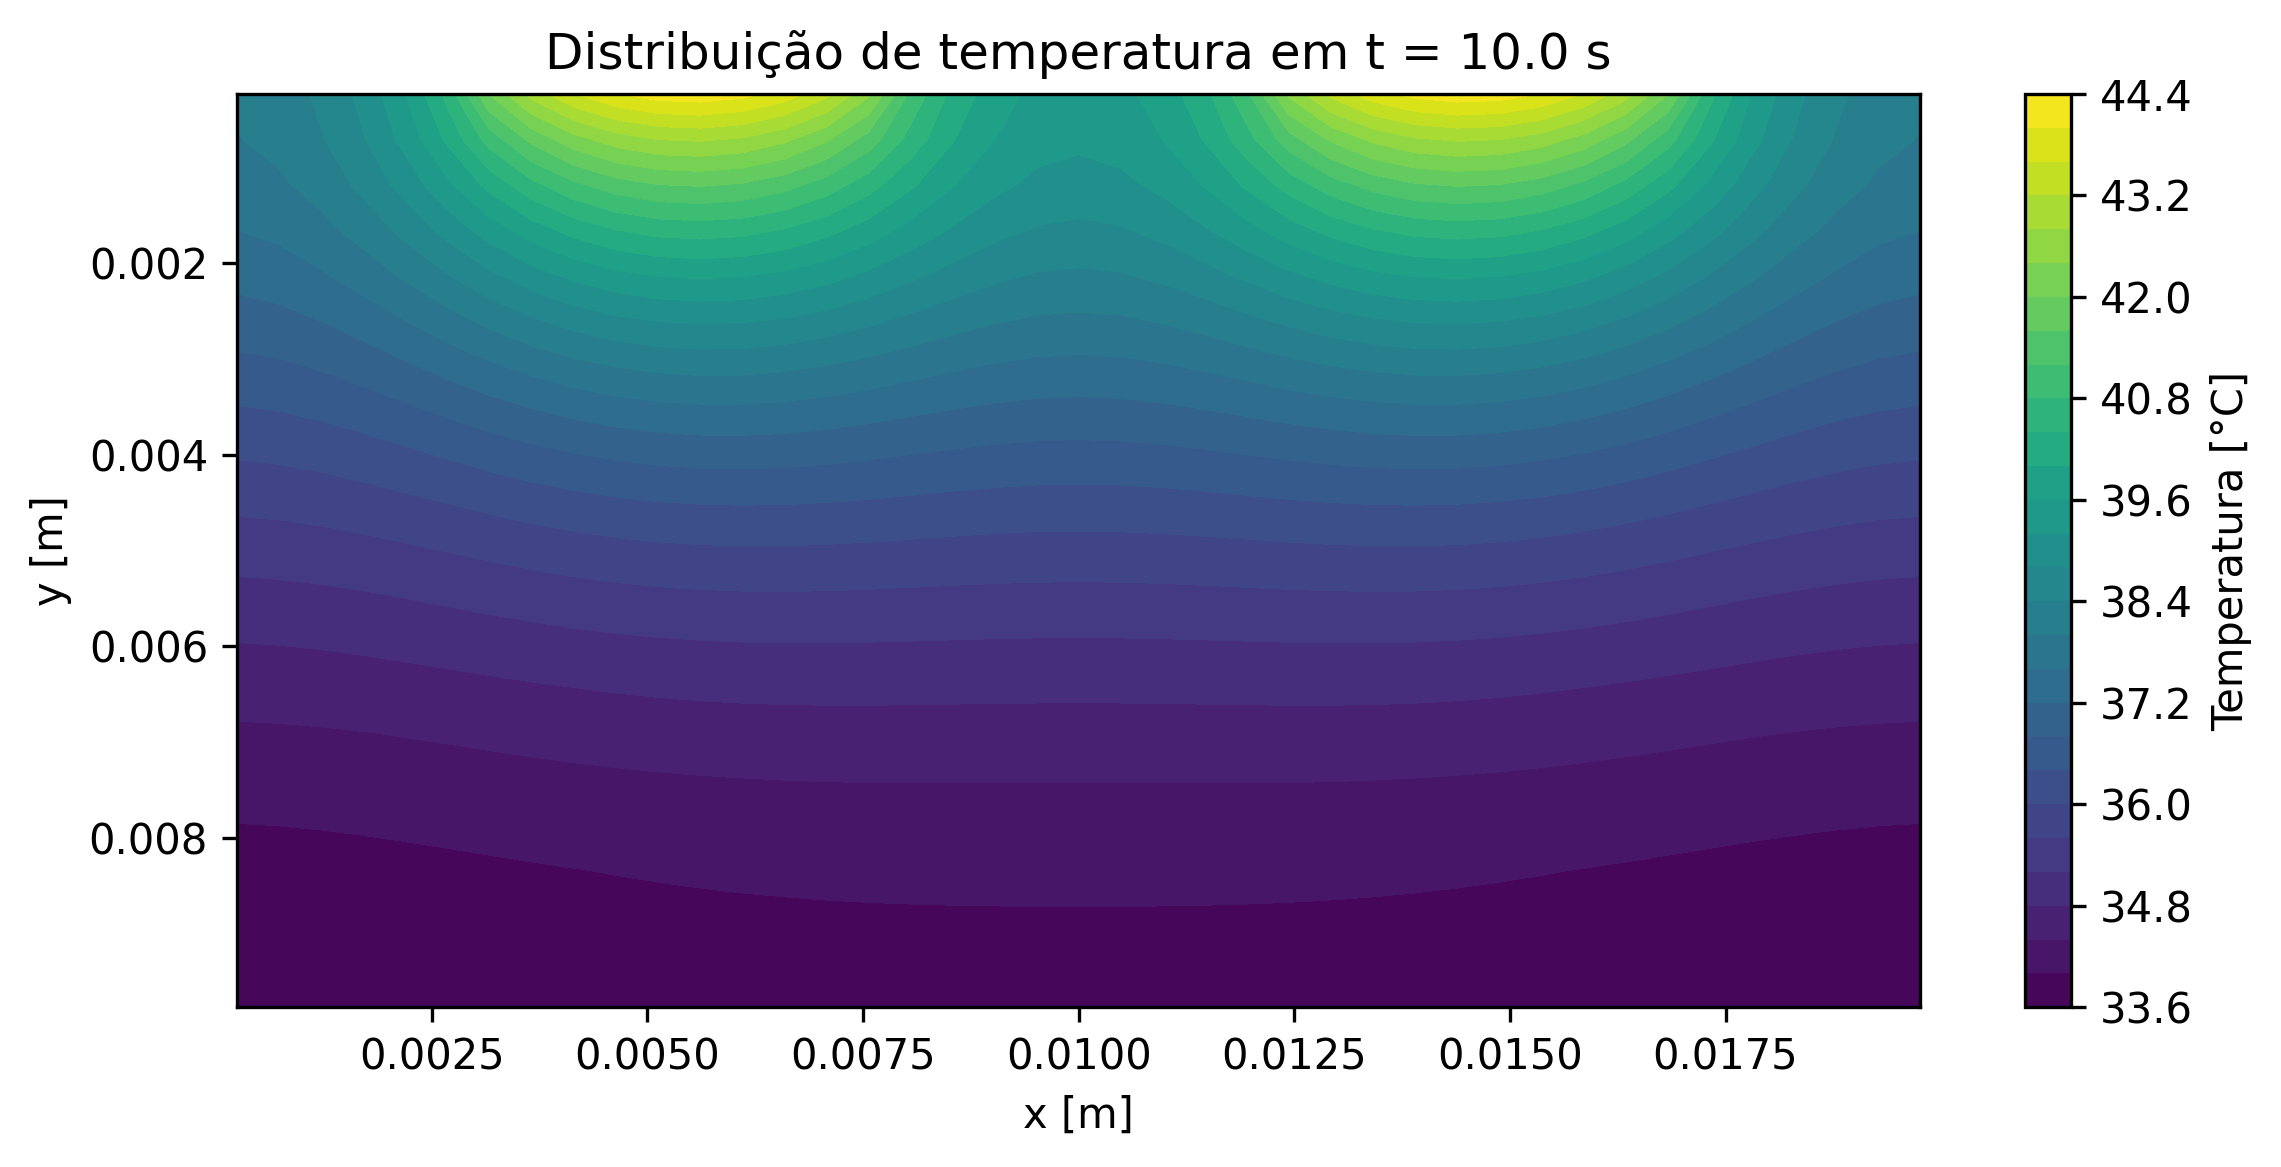
\includegraphics[width=0.78\textwidth]{figuras/campo_temperatura_t_10.png}
    \caption{Campo de temperatura em $t=\SI{10}{s}$.}
    \label{fig:t10}
\end{figure}

\begin{figure}[H]
    \centering
    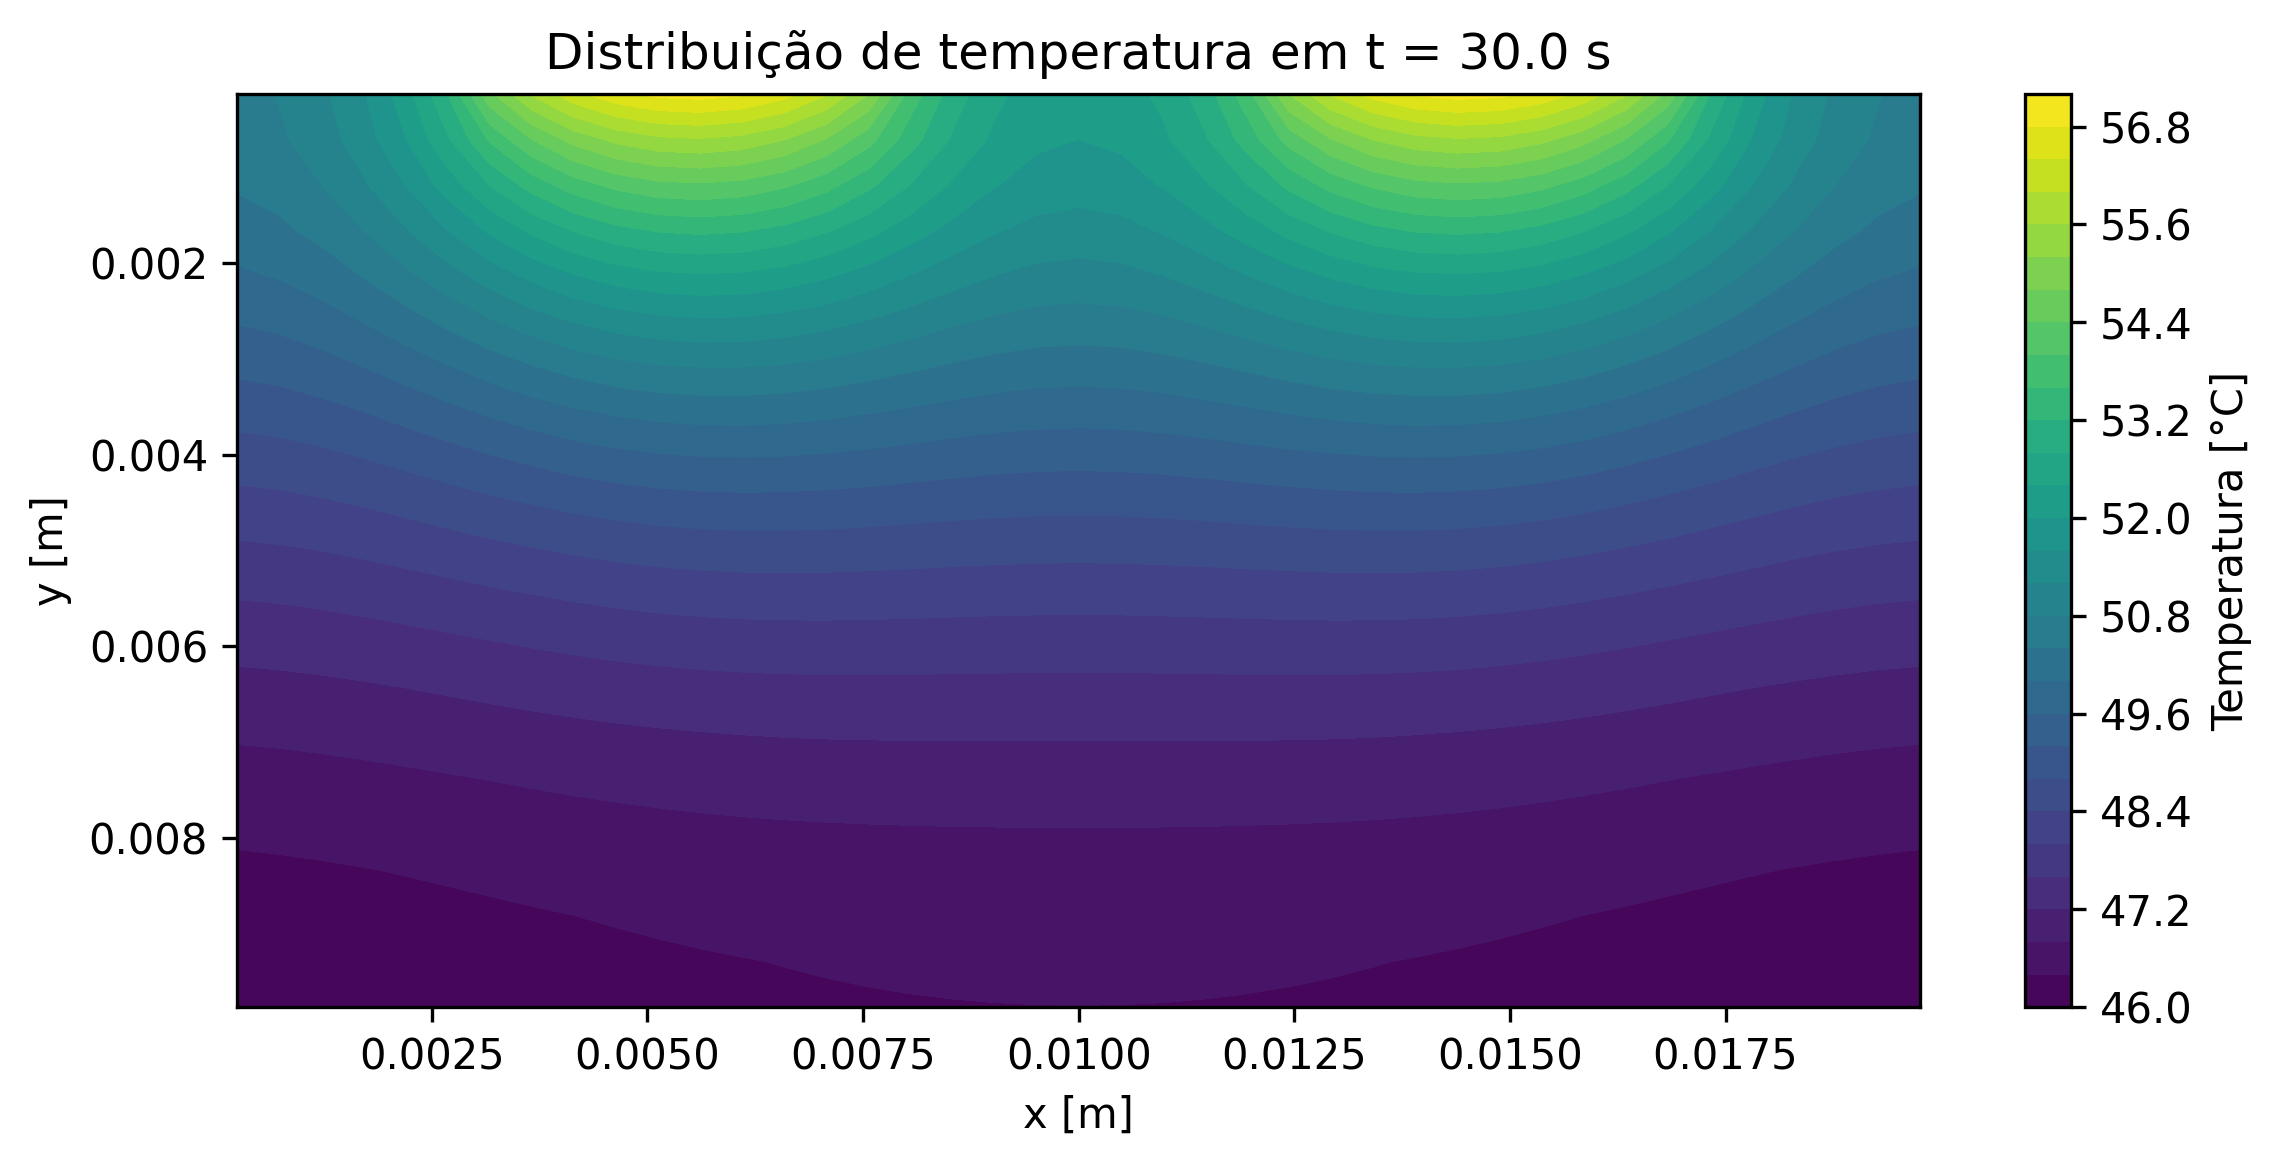
\includegraphics[width=0.78\textwidth]{figuras/campo_temperatura_t_30.png}
    \caption{Campo de temperatura em $t=\SI{30}{s}$.}
    \label{fig:t30}
\end{figure}

\begin{figure}[H]
    \centering
    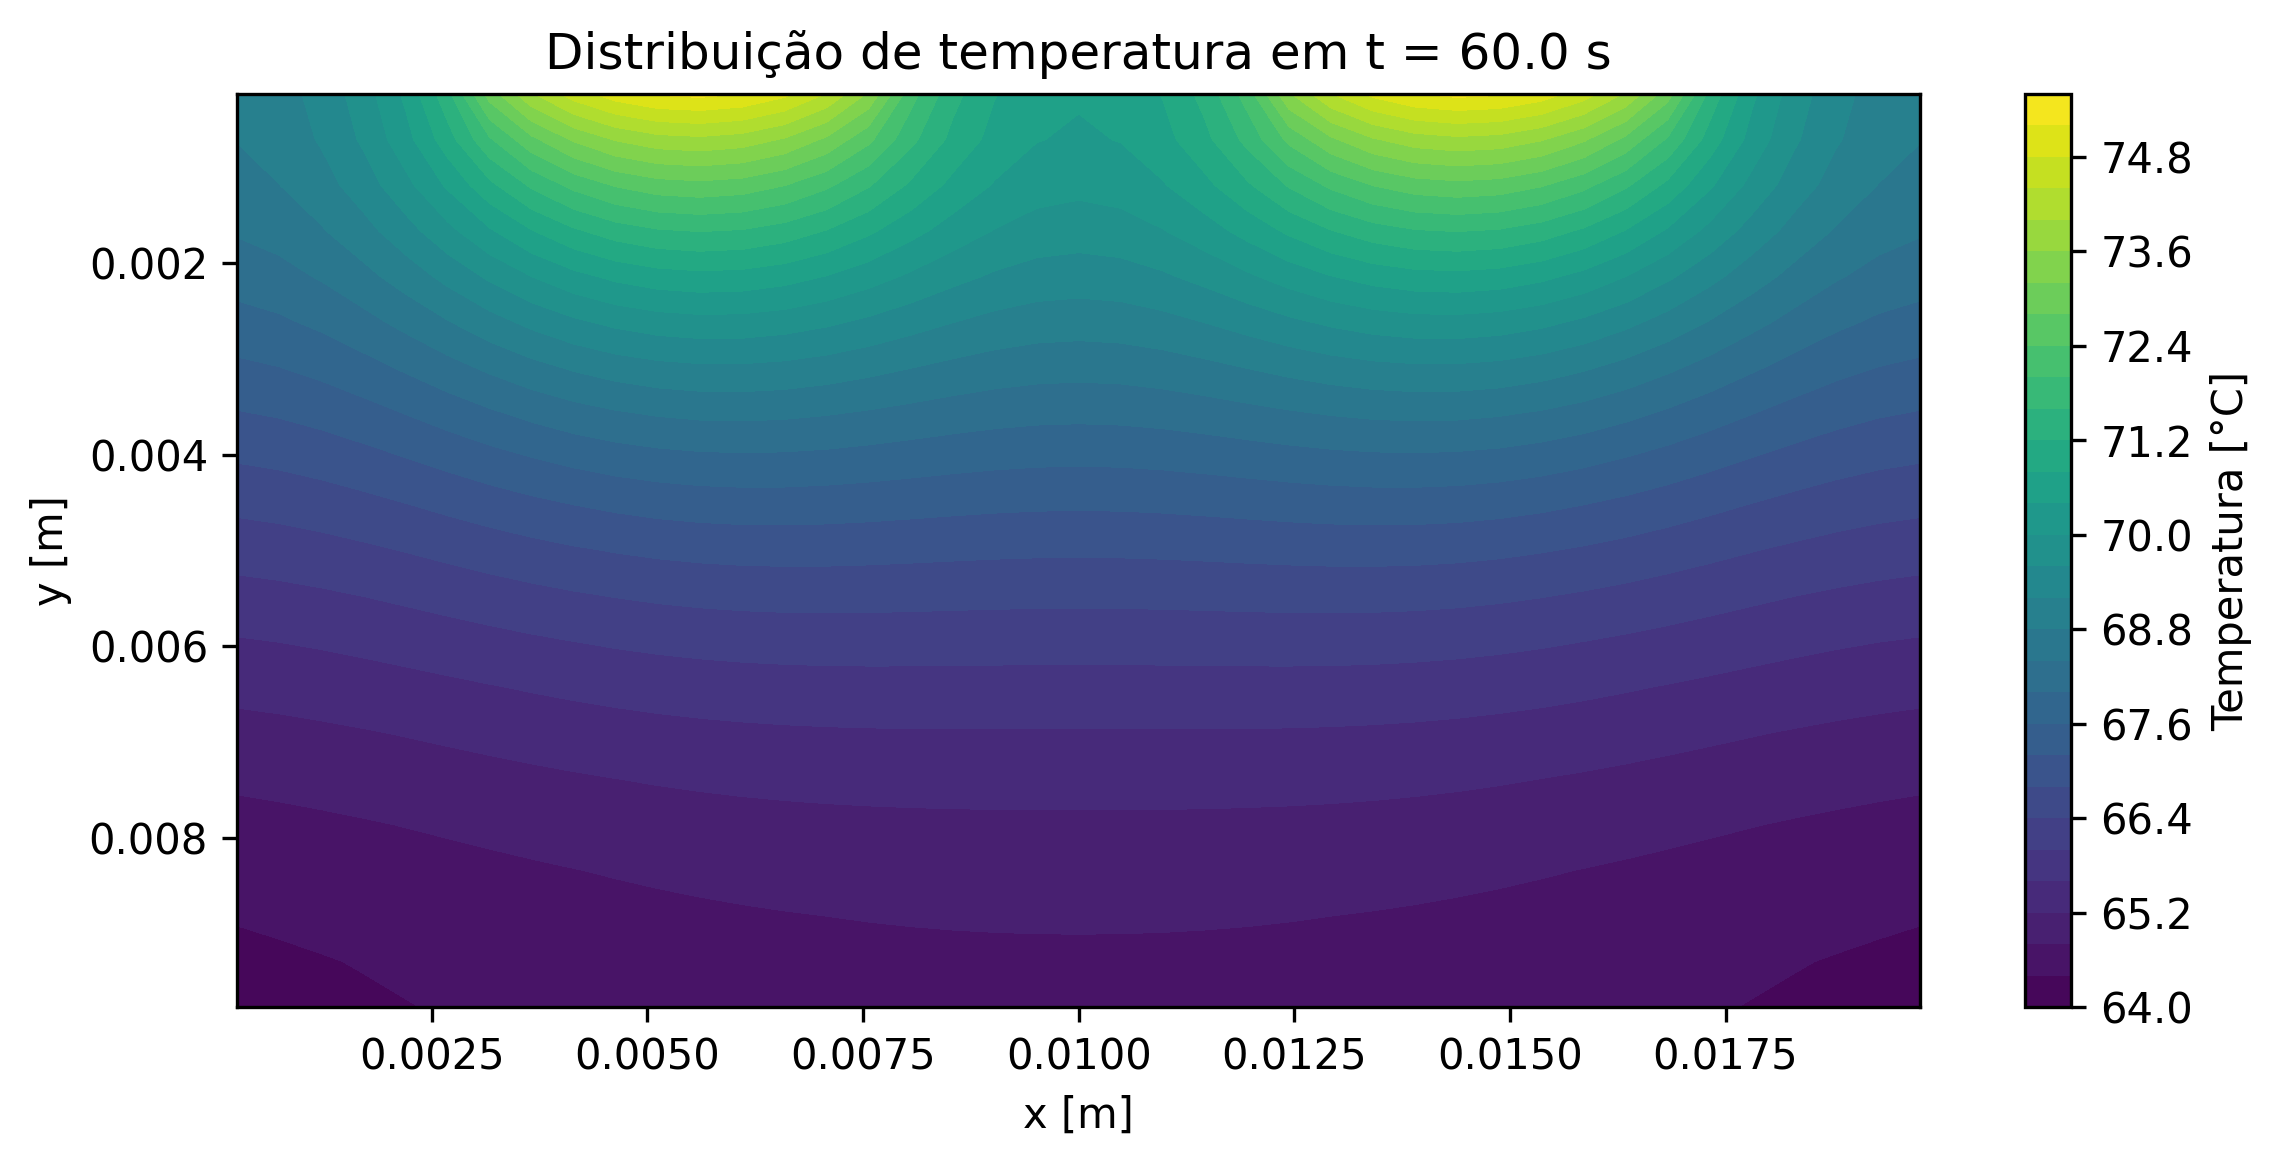
\includegraphics[width=0.78\textwidth]{figuras/campo_temperatura_t_60.png}
    \caption{Campo de temperatura em $t=\SI{60}{s}$.}
    \label{fig:t60}
\end{figure}

\section{Comentários finais}
Como o método de volumes finitos trabalha com temperaturas nos centros dos volumes de controle, os pontos exatamente sobre as bordas são aproximados pelo centro de volume mais próximo. Isso é numericamente consistente e suficiente para fins de análise da resposta térmica da chapa.

A formulação implícita foi adotada por sua robustez em problemas transientes, permitindo passos de tempo relativamente maiores sem instabilidade numérica. O recurso de uso opcional da GPU foi incorporado apenas como aceleração adicional; a solução permanece totalmente funcional em modo serial na CPU.

\end{document}
